\chapter[Tracking and Transfer Map Calculations]
{Bmad\_Standard and Symp\_Lie\_Bmad Tracking and Transfer Map Calculations}
\label{c:bmad.std}

For tracking and transfer map calculations (here generically called
``tracking''), \bmad has various methods that can be applied to a
given element (Cf. Chapter~\sref{c:methods}). This chapter discusses
the \vn{bmad_standard} calculation that is the default for almost all
element types and the \vn{symp_lie_bmad} calculation that does
symplectic integration.

Generally it will be assumed that tracking is in the forward direction.

%-------------------------------------------------------------------------
%-------------------------------------------------------------------------
\section{Tracking with Non-Zero Offsets, Pitches, or Tilt}
\label{s:misalign.track}

\index{element reference coordinates}
The general procedure for tracking through an element makes use of the
\vn{element reference coordinates} Without any offsets, pitches or
tilt, (henseforth called ``misalignments''), the element reference
coordinates are the same as the \vn{laboratory reference coordinates}
(\sref{s:ref}). With misalignments, the \vn{element reference
coordinates} will stay fixed relative to the element and will
therefore shift as the element shifts in the laboratory fram.

\index{crystal}\index{mirror}\index{multilayer_mirror}
For \vn{crystal} (\sref{s:crystal}), \vn{mirror} (\sref{s:mirror}),
and \vn{multilayer_mirror} (\sref{s:multilayer}) elements, the
non-straight reference trajectory through the element complicates the
calculation. For these elements, the \vn{element coordinates} is
choisen so that the $z$-axis points into the element as shown in
\fig{f:photon.ele.coords}.

Tracking a particle through an element is therefore a three
step transformation:
\begin{enumerate}
\item
At the entrance end of the element, transform from the
laboratory reference coordinates to the (entrance) \vn{element coordinates}.
\item
Track through the element ignoring any misalignments. For \vn{crystal}
and \vn{mirror} elements, this includes the transformation from
\vn{entrance} to \vn{exit element coordinates}.
\item
At the exit end of the element, transform from the \vn{element
reference from} to the \vn{laboratory reference frame}.
\end{enumerate}

The transformation between \vn{local} and \vn{element} reference frames
will depend upon whether \vn{local} reference frame through the
element is straight or not. 

\begin{figure}[tb]
  \centering
  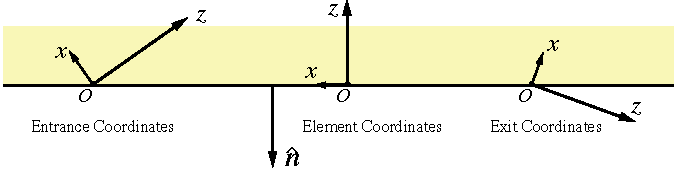
\includegraphics[width=5in]{photon-ele-coords.pdf}
  \caption[Crystal, Mirror, and Multilayer_Mirror Element Coordinates.]
{Element coordinates for \vn{crystal} (Bragg configuration),
\vn{mirror}, and \vn{multilayer_mirror} elements. The laboratory
entrance and exit coordinates are shown as well (assuming no
misalignments). In actuality, the origin $\Bf O$ of all three are the
same.  $\bfhat n$ is the normal to the element surface.}
  \label{f:photon.ele.coords}.
\end{figure}

%-------------------------------------------------------------------------
%-------------------------------------------------------------------------
\section{Transformation for Straight Elements Between 
Laboratory and Element Coordinates}
\label{s:straight.lab.ele}

It is assumed that pitches are are small so that second
order terms can be ignored.

%-------------------------------------------------------------------------
\subsection{Straight Transform from Laboratory to Element Coordinates}

The transformation from the laboratory coordinates to
element coordinates for an element that has a
straight reference trajectory through it is accomplished in a number of steps.
\begin{enumerate}
\item
Track as in a drift a distance \vn{z_offset_tot}.
\item
Apply offsets and pitches
\begin{align}
  x_1    &= x_0 - x_{\mbox{off}} + \frac{L}{2} x'_{pitch} \CRNO
  p_{x1} &= p_{x0} - (1 + p_{z0}) \, x'_{pitch} \CRNO
  y_1    &= y_0 - y_{\mbox{off}} + \frac{L}{2} y'_{pitch} \\
  p_{y1} &= p_{x0} - (1 + p_{z0}) \, y'_{pitch} \CRNO
  z_1    &= z_0 + x'_{pitch} \, x_1 + y'_{pitch} \, y_1 - 
    \frac{L}{4} (x^{\prime2}_{pitch} + y^{\prime2}_{pitch}) \nonumber
\end{align}
Notice that $z_1$ is written in terms of $x_1$ and $y_1$
\item
Apply any tilt $\theta_t$
\begin{align}
  x_2    &=  x_1    \, \cos\theta_t + y_1    \, \sin\theta_t \CRNO
  p_{x2} &=  p_{x1} \, \cos\theta_t + p_{y1} \, \sin\theta_t \CRNO
  y_2    &= -x_1    \, \sin\theta_t + y_1    \, \cos\theta_t \\
  p_{y2} &= -p_{x1} \, \sin\theta_t + p_{y1} \, \cos\theta_t \nonumber
\end{align}
\end{enumerate}

%-------------------------------------------------------------------------
\subsection{Straight Transform from Element to Laboratory Coordinates}

The back transformation from element to laboratory coordinates is
accomplished by the transformation
\begin{enumerate}
\item
Apply any tilt $\theta_t$
\begin{align}
  x_1    &=  x_0    \, \cos\theta_t - y_0    \, \sin\theta_t \CRNO
  p_{x1} &=  p_{x0} \, \cos\theta_t - p_{y0} \, \sin\theta_t \CRNO
  y_1    &=  x_0    \, \sin\theta_t + y_0    \, \cos\theta_t \\
  p_{y1} &=  p_{x0} \, \sin\theta_t + p_{y0} \, \cos\theta_t \nonumber
\end{align}
\item
Apply offsets and pitches
\begin{align}
  x_2    &= x_1 + x_{\mbox{off}} + \frac{L}{2} x'_{pitch}     \CRNO
  p_{x2} &= p_{x1} + (1 + p_{z1}) \, x'_{pitch}        \CRNO
  y_2    &= y_1 + y_{\mbox{off}} + \frac{L}{2} y'_{pitch}     \\
  p_{y2} &= p_{x1} + (1 + p_{z1}) \, y'_{pitch}        \CRNO
  z_2    &= z_1 + x'_{pitch} \, x_1 + y'_{pitch} \, y_1 - 
    \frac{L}{4} (x^{\prime2}_{pitch} + y^{\prime2}_{pitch})      \nonumber
\end{align}
\item
Track as in a drift a distance \vn{-z_offset_tot}.
\end{enumerate}


%-------------------------------------------------------------------------
%-------------------------------------------------------------------------
\section[Mirror and Crystal Element Transformation]
{Transformation for Mirror and Crystal Elements Between 
Laboratory and Element Coordinates}
\label{s:photon.lab.ele}

\index{mirror}\index{crystal}
It is assumed that pitches are are small so that second
order terms can be ignored.

%-------------------------------------------------------------------------
\subsection{Transformation from Laboratory to Element Coordinates}
\label{ss:crystal.trans.le}

\index{z_offset_tot}
With photons, the intensities must also be transformed.
The transformation from the the entrance laboratory coordinates to
the entrance element coordinates is:
\begin{enumerate}
\item
Track as in a drift a distance \vn{z_offset_tot}.
\item
\index{x_offset}\index{x_pitch}\index{y_offset}\index{y_pitch}
Apply offsets and pitches: The effective ``length'' of the element is
zero (\sref{s:mirror.coords}) so the origin of the element coordinates
is the same point around which the element is pitched so
\begin{align}
  x_1    &= x_0 - x_{\mbox{off}} \CRNO
  p_{x1} &= p_{x0} - (1 + p_{z0}) \, x'_{pitch} \CRNO
  y_1    &= y_0 - y_{\mbox{off}} \\
  p_{y1} &= p_{x0} - (1 + p_{z0}) \, y'_{pitch} \CRNO
  z_1    &= z_0 + x'_{pitch} \, x_1 + y'_{pitch} \, y_1 \nonumber
\end{align}
where $x_{\mbox{off}} \equiv \vn{x_offset}$, $x'_{pitch} \equiv \vn{x_pitch}$, etc.
\item
Apply \vn{ref_tilt} and \vn{tilt}:
\begin{align}
  \begin{pmatrix} x_2 \\ y_2 \end{pmatrix} &=
    \bfR (\theta_{tot}) \,   
  \begin{pmatrix} x_1 \\ y_1 \end{pmatrix} \CRNO
  \begin{pmatrix} p_{x2} \\ p_{y2} \end{pmatrix} &=
    \bfR (\theta_{tot}) \, 
  \begin{pmatrix} p_{x1} \\ p_{y1} \end{pmatrix} \label{xyrtxy} \\ 
  \begin{pmatrix} \bfE_{x2} \\ \bfE_{y2} \end{pmatrix} &=
    \bfR (\theta_{tot}) \,   \begin{pmatrix} \bfE_{x1} \\ \bfE_{y1} \end{pmatrix} \nonumber
\end{align}
where $\bfE$ is shorthand notation for
\Begineq
  \bfE \equiv E \, e^{i \, \phi}
\Endeq
with $E$ being the field intensity and $\phi$ being the field phase angle.
In the above equations $\bfR$ is the rotation matrix
\Begineq
  \bfR(\theta) = \begin{pmatrix} \cos\theta & \sin\theta \\ -\sin\theta & \cos\theta \end{pmatrix}
\Endeq
\index{tilt}\index{ref_tilt}\index{tilt_corr}
with $\theta_{tot}$ being 
\Begineq
  \theta_{tot}  = 
  \begin{cases}
    \vn{ref_tilt} + \vn{tilt} + \vn{tilt_corr} & \vn{for crystal elements} \\
    \vn{ref_tilt} + \vn{tilt} & \vn{for mirror elements}
  \end{cases}
  \label{tttt}
\Endeq
The \vn{tilt_corr} correction is explained in \sref{ss:crystal.trans}.
\end{enumerate}

%-------------------------------------------------------------------------
\subsection{Transformation from Element to Laboratory Coordinates}
\label{ss:crystal.trans.el}

The back transformation from exit element coordinates to exit
laboratory coordinates is accomplished by the transformation
  \begin{enumerate}
  \item
Apply \vn{ref_tilt} and \vn{tilt}: \vn{ref_tilt} rotates the exit
laboratory coordinates with respect to the exit element coordinates in
the same way \vn{ref_tilt} rotates the entrance laboratory coordinates
with respect to the entrance element coordinates. The forward and back
transformations are thus just inverses of each other.  With
\vn{tilt}, this is not true. \vn{tilt}, unlike \vn{ref_tilt}, does
not rotate the output laboratory coordinates.  There is the further
complication in that \vn{tilt} is a rotation about the {\em
entrance} laboratory coordinates. The first step is to express
\vn{tilt} with respect to the exit coordinates. This is done with
the help of the $\bfS$ matrix of \Eq{ltl} with $\alpha$ given by
\Eq{agg}. The effect of the \vn{tilt} can be modeled as a rotation
vector $\Bf e_{in}$ in the entrance laboratory coordinates pointing
along the $z$-axis
\Begineq
 \Bf e_{in} = (0, 0, \mbox{tilt})
\Endeq
In the exit laboratory coordinates, the vector $\Bf e_{out}$ is
\Begineq
  \Bf e_{out} = \bfS \, \Bf e_{in}
\Endeq
The $z$ component of $\Bf e_{out}$ combines with \vn{ref_tilt} to give
the transformation
\begin{align}
  \begin{pmatrix} x_2 \\ y_2 \end{pmatrix} &=
    \bfR (-\theta_{t}) \,   \begin{pmatrix} x_1 \\ y_1 \end{pmatrix} \CRNO
  \begin{pmatrix} p_{x2} \\ p_{y2} \end{pmatrix} &=
    \bfR (-\theta_{t}) \,   \begin{pmatrix} p_{x1} \\ p_{y1} \end{pmatrix} \\
  \begin{pmatrix} \bfE_{x2} \\ \bfE_{y2} \end{pmatrix} &=
    \bfR (-\theta_{t}) \,   \begin{pmatrix} \bfE_{x1} \\ \bfE_{y1} \end{pmatrix} \nonumber
\end{align}
where $\theta_t$ is $\mbox{ref_tilt} + \Bf e_{out,z}$. The $x$ and $y$ components
of $\Bf e_{out}$ give rotations around the $x$ and $y$ axes
\begin{align}
  p_{x3} &= p_{x2} - \Bf e_{out,y} \CRNO
  p_{y3} &= p_{y2} + \Bf e_{out,x} \\
  z_3    &= z_2 + x_2 \, \Bf e_{out,y} - y_2 \, \Bf e_{out,x}
\end{align}
  \item
Apply pitches: Since pitches are defined with
respect to the entrance laboratory coordinates, they have to be
translated to the exit laboratory coordinates
\Begineq
  \bfP_{out} = \bfS \, \bfP_{in}
\Endeq
where $\bfP_{in} = (x'_{pitch}, y'_{pitch}, 0)$ is the pitch vector in
the entrance laboratory frame and $\bfP_{out}$ is the vector in the exit
laboratory frame. The transformation is then
\begin{align}
  p_{x4} &= p_{x3} - \bfP_{out,y} \CRNO
  p_{y4} &= p_{y3} + \bfP_{out,x} \\
  z_4    &= z_3 + x_3 \, \bfP_{out,y} - y_3 \, \bfP_{out,x}
\end{align}
  \item
Apply offsets: Again, offsets are defined with respect to the
entrance laboratory coordinates. Like pitches, the translation is
\Begineq
  \bfO_{out} = \bfS \, \bfO_{in}
\Endeq
where $\bfO_{in} = (x_{\mbox{off}}, y_{\mbox{off}}, s_{\mbox{off}})$ is the offset in the
entrance laboratory frame. The transformation is
\begin{align}
  x_5 &= x_4 + \bfO_{out,x} - p_{x4} \, \bfO_{out,z} \CRNO
  y_5 &= y_4 + \bfO_{out,y} - p_{y4} \, \bfO_{out,z} \\
  z_5 &= z_4 + \bfO_{out,z} 
\end{align}
  \end{enumerate}

%-------------------------------------------------------------------------

\begin{figure}[tb]
  \centering
  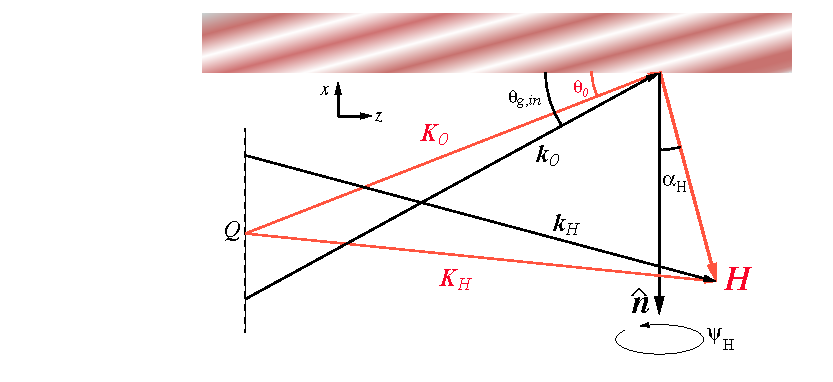
\includegraphics[width=5in]{crystal-diffraction.pdf}
  \caption[Reference trajectory reciprocal space diagram for crystal diffraction.]
{Reference trajectory reciprocal space diagram for for A) Bragg
diffraction and B) Laue diffraction. The bar over the vectors
indicates that they refer to the reference trajectory. The $x$-$z$
coordinates shown are the element body coordinates. All points in the
diagram are in the plane of the paper except for the tip of $\bfH$.
$\bfKbar_{0}$, and $\bfKbar_{H}$ are the wave vectors inside the
crystal and $\bfkbar_{0}$ and $\bfkbar_{H}$ are the wave vectors
outside the crystal. The reference photon traveling along the
reference trajectory has $\bfKbar_0$ and $\bfKbar_H$ originating at
the $Q$ point. For Laue diffraction, the crystal faces are assumed
parallel.  For Bragg diffraction the crystal normal is in the $-\bfhat
x$ direction while for Laue diffraction the crystal normal is in the
$-\bfhat z$ direction
  }
  \label{f:crystal.diffraction}
\end{figure}

%-------------------------------------------------------------------------
%-------------------------------------------------------------------------
\section{Crystal Element Tracking}
\label{s:crystal.tracking}

\textit{\large [Crystal tracking developed by Jing Yee Chee, Ken Finkelstein, and David Sagan]}

Crystal diffraction is modeled using dynamical diffraction theory. The
notation here follows Batterman and Cole\cite{b:batterman}.  The
problem can be divided up into two parts. First the reference
trajectory must be calculated. This means calculating the incoming
grazing angle $\theta_{B,in}$ and outgoing grazing angle
$\theta_{B,out}$ as well as calculating the transformations between
the various coordinate systems. This is done in \sref{ss:crystal.ref},
\sref{ss:crystal.trans}, and \sref{ss:crystal.dlaue}.  The second part
is the actual tracking of the photon and this is covered in
\sref{ss:crystal.track}.

%-------------------------------------------------------------------------
\subsection{Calculation of Entrance and Exit Bragg Angles}
\label{ss:crystal.ref}

\fig{f:crystal.diffraction} shows the geometry of the
problem. The bar over the vectors indicates that they refer to the
reference trajectory. The reference trajectory is calculated such that
the reference photon will be in the center of the Darwin curve. That
is, the internal wave vectors $\bfKbar_0$ and $\bfKbar_H$ originate
from the $Q$ point (See \cite{b:batterman} Figs.~8 and 29).

The external wave vectors $\bf k_0$, and $\bf k_H$ and the internal wave vectors
have magnitude
\begin{align}
  |\bf k_0| &= |\bf k_H| = \frac{1}{\lambda} 
  \label{kk1l1} \\
  |\bfKbar_0| &= |\bfKbar_H| = \frac{1}{\lambda \, (1 + \delta)}
  \label{kk1l2}
\end{align}
where $\lambda$ is the wavelength, and $\delta$ is
\Begineq
  \delta = \frac{\lambda^2 r_e}{2 \, \pi \, V} \, |F_0|
\Endeq
with $r_e$ being the classical electron radius, $V$ the unit cell
volume, and $F_0$ the $F_{(0,0,0)}$ structure factor. 

In element body coordinates (which will be the coordinate system used
henceforth), $\bfkbar_0$ lies in the $x$-$z$ plane. $\bfKbar_0$ is
related to $\bfkbar_0$ via Batterman Eq.~(25)
\Begineq
  \bfK_0 = \bfk_0 + q_0 \, \bfhat n
  \label{kkqn1}
\Endeq
where the value of $q_0$ is to be determined. Here, and in equations
below, if the equation is true in general, and not just for the
reference trajectory, the bar superscript is dropped.

Since $\bfhat n$ is in the $-\bfhat x$ direction, $\bfKbar_0$ is also
in the $x$-$z$ plane. Thus $\bfkbar_0$ and $\bfKbar_0$ can be written
in the form
\begin{alignat}{3}
  \bfkbar_0 &= \frac{1}{\lambda} \, 
    \begin{pmatrix}
    -\cos\theta_{B,in} \\
    0 \\
    \sin\theta_{B,in}
    \end{pmatrix}
  \; , & \qquad
  \bfKbar_0 &= \frac{1}{\lambda \, (1 + \delta)} \, 
    \begin{pmatrix}
    -\cos\theta_0 \\
    0 \\
    \sin\theta_0
    \end{pmatrix}
  & \qquad &\mbox{[Bragg]} \CRNO
  \bfkbar_0 &= \frac{1}{\lambda} \, 
    \begin{pmatrix}
    \sin\theta_{B,in} \\
    0 \\
    \cos\theta_{B,in}
    \end{pmatrix}
  \; , & \qquad
  \bfKbar_0 &= \frac{1}{\lambda \, (1 + \delta)} \, 
    \begin{pmatrix}
    \sin\theta_0 \\
    0 \\
    \cos\theta_0
    \end{pmatrix}
  &\qquad & \mbox{[Laue]} 
  \label{k1lst}
\end{alignat}
Where, as shown in \fig{f:crystal.diffraction}, $\theta_{B,in}$, and
$\theta_0$ are the angles of $\bfkbar_0$ and $\bfKbar_0$ with respect
to the $x$-axis for Bragg reflections and with respect to the $z$-axis
for Laue reflection.

$\alpha_H$ (\vn{alpha_angle}) is the angle that $\bfH$ makes with
respect to the $-\bfhat z$ axis and $\psi_H$ (\vn{psi_angle}) is the
rotation of $\bfH$ around the $-\bfhat z$ axis such that for $\psi_H =
0$, $\bfH$ is in the $x$-$z$ plane and oriented as shown in
\fig{f:crystal.diffraction}. Thus
\Begineq
  \bfH 
  \equiv \frac{1}{d} \, \bfhat{H} 
  = \frac{1}{d}
    \begin{pmatrix} 
       -\sin \alpha_H \, \cos \psi_H \\ \sin \alpha_H \, \sin \psi_H \\ -\cos \alpha_H
    \end{pmatrix}
  \label{h1daa}
\Endeq
where $\bfhat{H}$ is $\bfH$ normalized to 1.

The vectors $\bfK_0$ and $\bfH$ must add up to the reciprocal lattice vector $\bfK_H$
\Begineq
  \bfK_H = \bfK_0 + \bfH
  \label{kkh}
\Endeq
Taking the length of both sides of this equation and using
\Eqs{kk1l2}, \eq{k1lst}, and \eq{h1daa} gives for
$\theta_0$
\Begineq
  \sin \theta_0 = 
  \begin{dcases}
    \dsfrac{-\beta \, \what{H}_z - \what{H}_x \, \sqrt{\what{H}_x^2 + \what{H}_z^2 - \beta^2}}
    {\what{H}_x^2 + \what{H}_z^2} & \vn{Bragg} \\
    \dsfrac{-\beta \, \what{H}_x + \what{H}_z \, \sqrt{\what{H}_x^2 + \what{H}_z^2 - \beta^2}}
    {\what{H}_x^2 + \what{H}_z^2} & \vn{Laue}
  \end{dcases}
\Endeq
where
\Begineq
  \beta \equiv \frac{\lambda \, (1 + \delta)}{2 \, d}
\Endeq
Once $\theta_0$ has been calculated, $\theta_{B,in}$ can be calculated from \Eq{kkqn1}
\begin{align}
  \cos\theta_{B,in} &= \frac{\cos\theta_0}{1 + \delta} \quad [\mbox{Bragg}] \\
  \sin\theta_{B,in} &= \frac{\sin\theta_0}{1 + \delta} \quad [\mbox{Laue}] 
\end{align}

The outgoing reference wave vector $k_H$ is computed using the equation
\Begineq
  \bfK_H = \bfk_H + q_H \, \bfhat n
  \label{kkqn2}
\Endeq
Using this with \Eqs{h1daa} and \eq{kkh} gives
\begin{align}
  \kbar_{H,x} &= \Kbar_{H,z} = \frac{1}{d} \, \what{H}_x + \kbar_{0,x} \\
  \kbar_{H,y} &= \Kbar_{H,y} = \frac{1}{d} \, \what{H}_y 
  \label{k1dapl} \\
  \kbar_{H,z} &= \sqrt{\frac{1}{\lambda^2} - \kbar_{H,x}^2 - \kbar_{H,y}^2} \nonumber
\end{align}

The total bending angle of the reference trajectory is then
\Begineq
  \theta_{bend} = \tan^{-1} 
  \left( \frac{ | \bfkbar_0 \times \bfkbar_H | }{\bfkbar_0 \cdot \bfkbar_H} \right)
\Endeq
The outgoing Bragg angle $\theta_{B,out}$ is then {\em defined} to be
the difference between the total bend angle and the entrance Bragg angle.
\Begineq
  \theta_{B,out} \equiv \theta_{bend} - \theta_{B,in}
\Endeq

%-------------------------------------------------------------------------
\subsection{Crystal Coordinate Transformations}
\label{ss:crystal.trans}

There are four transformations needed between coordinates
denoted by $\Bf\Sigma_1$, $\Bf\Sigma_2$, $\Bf\Sigma_3$, and $\Bf\Sigma_4$
\begin{example}
  \(\Bf\Sigma_1\)  Transform from laboratory entrance to element entrance coordinates.  
  \(\Bf\Sigma_2\)  Transform from element entrance to body coordinates.  
  \(\Bf\Sigma_3\)  Transform from body to element exit coordinates.  
  \(\Bf\Sigma_4\)  Transform from element exit to laboratory exit coordinates.  
\end{example}
The total transformation is just the map represented by $\bfS$ and
$\bfV$ of \Eqs{vwlv} and \eq{wws}
\Begineq
  [\bfS, \bfV] = \Bf\Sigma_4 \, \Bf\Sigma_3 \, \Bf\Sigma_2 \, \Bf\Sigma_1
\Endeq

\index{tilt_corr}\index{crystal!tilt correction}
The transformation $\Bf\Sigma_1$ is given in
\sref{ss:crystal.trans.le} and the transformation $\Bf\Sigma_4$ is
given in \sref{ss:crystal.trans.el}. In general, the transformation
$\Bf\Sigma_1$ needs a ``tilt correction'' (\Eq{tttt}), as explained
below, when $\psi_H$ is nonzero.  The exception is that in the case
when the non-diffracted beam is tracked in Laue diffraction, no tilt
correction is needed. Since this tilt correction is
independent of any misalignments, the tilt correction calculation
proceeds assuming here that there are no misalignments. The finite
$\bfV$ due to the finite crystal thickness in Laue diffraction will
also be ignored for the moment.

Without misalignments, and with $\psi_H$ zero, the transformation
$\Bf\Sigma_1$ is, as it is for every other type of element,
just the unit matrix. 
\Begineq
  \Bf\Sigma_1 = \bfI
\Endeq
That is, the two coordinate systems are
identical. Furthermore, the transformation $\Bf\Sigma_2$ from element
entrance coordinates to body coordinates is a rotation around the $y$
axis
\Begineq
  \Bf\Sigma_2 = \bfR_y(\theta_{B,in}) \equiv \begin{pmatrix}
     \cos\theta_{B,in} & 0 & \sin\theta_{B,in} \\
     0                 & 1 & 0                 \\
    -\sin\theta_{B,in} & 0 & \cos\theta_{B,in} \\
  \end{pmatrix}
  \label{mt0t010}
\Endeq
The transformation from element body coordinates to element exit
coordinates, $\Bf\Sigma_3$, is another rotation around the $y$ axis 
\Begineq
  \Bf\Sigma_3 = \bfR_y(\theta_{B,out})
\Endeq
and the transformation from element exit coordinates
to laboratory exit coordinates, $\Bf\Sigma_{out}$ is the unity matrix
\Begineq
  \Bf\Sigma_4 = \bfI
\Endeq
Thus, the combined transformation $\bfS$ from laboratory entrance to
laboratory exit coordinates is a rotation around the $y$ axis of
$\theta_{B,in}+\theta_{B,out}$ as explained in section
\sref{s:global}
\Begineq
  \bfS = \Bf\Sigma_4 \, \Bf\Sigma_3 \, \Bf\Sigma_2 \, \Bf\Sigma_1 
  = \bfR_y(\theta_{B,in}+\theta_{B,out})
\Endeq

\index{ref_tilt}\index{psi_angle}
When $\psi_H$ is non-zero, the situation is complicated since, if
$\bfS$ as calculated above is used, the vector $\bfkbar_H$ would be
bent out of the $x$-$z$ plane even though it has been assumed that the
\vn{ref_tilt} $\theta_t$ is zero. But $\bfkbar_H$ points in the same direction
as the $z$ axis of the outgoing reference trajectory. Furthermore, by
{\em definition}, the reference trajectory has the form given by
\Eq{lrca1} with the $\bfT$ matrix depending only upon the \vn{ref_tilt}
parameter (which is here taken to be zero). To satisfy \Eq{lrca1}, the
crystal must be reorientated to keep the $\bfk_H$ vector in the
$x$-$z$ plane of the laboratory entrance coordinates.  The
reorientation is done by rotating the crystal about the laboratory
entrance $\Bf z$ axis by an amount $\theta_{corr}$ (\vn{tilt_corr}).

With this tilt correction the transformation $\Bf\Sigma_1$ is a
rotation about the $z$ axis
\Begineq
  \Bf\Sigma_1 = 
  \begin{pmatrix}
    \cos\theta_{corr} & -\sin\theta_{corr} & 0 \\
    \sin\theta_{corr} &  \cos\theta_{corr} & 0 \\
    0                 &  0                 & 1                
  \end{pmatrix}
\Endeq
To calculate a value for $\theta_{corr}$, note that
the transformation $\Bf\Sigma_2$ from element entrance coordinates to element body
coordinates is not affected by a finite $\psi_H$ and so \Eq{mt0t010}
is unmodified. The $\bfk_H$ vector, expressed in laboratory entrance
coordinates, is $\Bf\Sigma_1^{-1} \, \Bf\Sigma_2^{-1} \, \bfk_H$ where the
components of $\bfk_H$ are given by \Eq{k1dapl}. To
satisfy \Eq{lrca1}, this vector must have zero $y$ component
\Begineq
  \left( \Bf\Sigma_1^{-1} \, \Bf\Sigma_2^{-1} \, \bfk_H \right) \cdot
  \begin{pmatrix} 0 \\ 1 \\ 0 \end{pmatrix}
  = 0
\Endeq
Solving gives
\Begineq
  \theta_{corr} = \tan^{-1} 
  \frac{k_{H,y}}{k_{H,z} \, \sin\theta_{B,in} - k_{H,x} \, \cos\theta_{B,in}}
\Endeq
The transformation $\Bf\Sigma_3$ from element body coordinates to
element exit coordinates is now obtained by requiring that the total
transformation from laboratory entrance to laboratory exit coordinates
be the $\bftilde S$ matrix given in \Eq{lrca1}
\Begineq
  \Bf\Sigma_3 \, \Bf\Sigma_2 \, \Bf\Sigma_1 = 
  \begin{pmatrix}
    \cos\theta_{bend} & 0 & -\sin\theta_{bend} \\
    0          & 1 & 0           \\
    \sin\theta_{bend} & 0 & \cos\theta_{bend}
  \end{pmatrix}
\Endeq
In the above equation, the transformation $\Bf\Sigma_4$ has been
dropped since it is the unit matrix independent of $\psi_H$.

For Laue diffraction when the non-diffracted beam is tracked, the exit
coordinate system corresponds to the entrance coordinate system. That
is, $\bfV$ is the unit matrix. In this case, there is no tilt
correction and $\Bf\Sigma_3 = \bfR_y(-\theta_{B,in})$ is just the
inverse of $\Bf\Sigma_2$.

%-------------------------------------------------------------------------

\begin{figure}
\centering
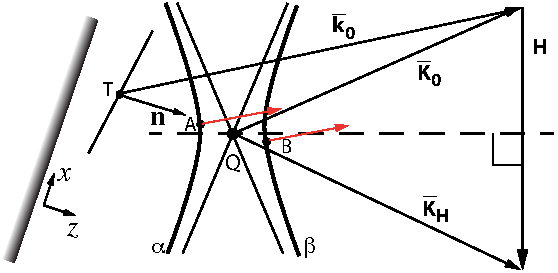
\includegraphics[width=4in]{crystal-energy.pdf}
  \caption[Energy flow for Laue diffraction]{
Energy flow for Laue diffraction.
  }
\label{f:crystal.energy}
\end{figure}

%-------------------------------------------------------------------------
\subsection{Laue Reference Orbit Displacement Vector}
\label{ss:crystal.dlaue}

For Laue diffraction, the reference orbit displacement vector $\bfL$ (cf.~\Eq{vwlv})
is nonzero due to the nonzero crystal thickness. The energy flow for
any tie point is perpendicular to the real part of the dispersion
curve at the point (\cite{b:batterman} $\S$2.9B). This is illustrated
in \fig{f:crystal.energy}. By symmetry, the energy flow for point
Q is perpendicular to $\bfH$. The energy flow for the reference curve
will thus be in the direction
\Begineq
  \bfS_{ref} \propto \bfKbar_{0H} \equiv \bfKbar_0 + \bfKbar_H
\Endeq
The reference orbit displacement vector is then
\Begineq
  \bfL = \frac{\bfKbar_{0H} \, ( \bfKbar_{0H} \cdot \Bf t )}{|\bfKbar_{0H}|^2}
\Endeq
where
\Begineq
  \Bf t = \begin{pmatrix}
    0 \\ 0 \\ t
  \end{pmatrix}
\Endeq
and $t$ is the crystal thickness.

%-------------------------------------------------------------------------
\subsection{Crystal Element Tracking}
\label{ss:crystal.track}


The starting photon coordinates are specified in the laboratory
entrance coordinates. The transformation from laboratory entrance
coordinates to element entrance coordinates $\bftilde k_0$ is given in
\sref{s:photon.lab.ele}. The transformation to element body
coordinates $\bfk_0$ is
\begin{equation}
  \bfk_0 =  \Bf\Sigma_2 \, \bftilde k_0
\end{equation}
with $\Bf\Sigma_2$ given by \Eq{mt0t010}.
The outgoing wave vector $\bfk_H$ is related to $\bfk_0$ via
\Begineq
  \bfk_H =  \bfk_0 + \bfH + q_t \, \bfhat n
\Endeq
where $q_t$ is determined by using \Eqs{k1lst} and \eq{h1daa} in \Eq{kk1l1}
\begin{align}
  k_{H,x} &= k_{0,x} + H_x \nonumber \CRNO
  k_{H,y} &= k_{0,y} + H_y \\
  k_{H,z} &= \sqrt{\lambda^2 - k_{H,x}^2 - k_{H,y}^2} \nonumber
\end{align}

To compute the field amplitude of the outgoing photon, the equation to
be solved is (\cite{b:batterman} Eq.~(21))
\Begineq
  \xi_0 \, \xi_H = \frac{1}{4} \, k^2 \, P^2 \, \Lambda^2 \, F_H \, F_{\bar H}
  \label{xx14}
\Endeq
where $\xi_0$ and $\xi_H$ are given by \cite{b:batterman} Eq.~(18)
and $P$ is the polarization factor
\Begineq
  P = 
  \begin{cases}
    1               & \sigma \mbox{ polarization state} \\
    \cos 2\theta_g  & \pi \mbox{ polarization state}
  \end{cases}
\Endeq
$2\theta_g$ is the angle between $\bfK_0$ and $\bfK_H$ which is well
approximated by $\theta_{B,in} + \theta_{B,out}$.

The solution to \Eq{xx14} is (\cite{b:batterman} Eq.~(31))
\begin{align}
  \xi_0 &= \frac{1}{2} \, k \, |P| \, \Gamma \, [F_H \, F_{\bar H}]^{1/2} \, 
    |b|^{1/2} \, [\eta \pm (\eta^2 + \sign(b))^{1/2}] \CRNO
  \xi_H &= \frac{1}{2} \, k \, |P| \, \Gamma \, [F_H \, F_{\bar H}]^{1/2} \, 
    \frac{1}{|b|^{1/2} \, [\eta \pm (\eta^2 + \sign(b))^{1/2}]}
\end{align}
where $\sign$ is the sign function
\Begineq
  \sign(b) \equiv \begin{cases} 1 & b > 0 \\ -1 & b < 0 \end{cases}
\Endeq
and $\eta$ is given by \cite{b:blasdell} Eq.~(5)
\Begineq
  \eta = \frac{-b \, a + \Gamma \, F_0 \, (1 - b)}{2 \, \Gamma \, |P| \, \sqrt{|b| \, F_H \, F_{\bar H}}}
\Endeq
with the asymmetry factor $b$ for the photon being tracked being given
by \cite{b:blasdell} Eq.~(3)
\Begineq
  b \equiv \frac{\bfhat n \cdot \bfhat k_0}{\bfhat n \cdot \widehat{{\bfk_0 + \bfH}}}
\Endeq
and the angular deviation variable $a$ is given by \cite{b:blasdell} Eq.~(4)
\Begineq
  a \equiv \frac{H^2 + 2 \, \bfk_0 \cdot \bfH}{k_0^2}
\Endeq
Once $\xi_0$ and $\xi_H$ are determined, the ratio of the incoming and outgoing fields
for the $\alpha$ or $\beta$ branches can be computed via (\cite{b:batterman} Eq.~(24))
\Begineq
  r \equiv \frac{E_H}{E_0} 
  = \frac{- \, 2 \, \xi_0}{k \, P \, \Gamma \, F_{\bar H}} \,
  = \, \frac{- \, k \, P \, \Gamma \, F_H}{2 \, \xi_H} 
\Endeq
where the $\alpha$ or $\beta$ subscript has been supressed.  The total
field which is the sum of the fields on the branches is computed using
the boundary conditions
\Begineq
  \bfE_0 = \bfE_{0\alpha} + \bfE_{0\beta}, \qquad\qquad 
  0 = \bfE_{H\alpha} + \bfE_{H\beta}
\Endeq
Using the above two equations gives
\begin{align}
  \bfE_{0\alpha} &= \bfE_0 \, \frac{r_\beta}{r_\beta - r_\alpha} \qquad\qquad
  \bfE_{H\alpha}  = \bfE_0 \, \frac{r_\alpha \, r_\beta}{r_\beta - r_\alpha} \CRNO
  \bfE_{0\beta} &= -\bfE_0 \, \frac{r_\alpha}{r_\beta - r_\alpha} \qquad\qquad
  \bfE_{H\beta}  = -\bfE_0 \, \frac{r_\alpha \, r_\beta}{r_\beta - r_\alpha} 
\end{align}

For Laue diffraction the photon has to be tracked from the entrance
surface to the exit surface. It is assumed that the two interior wave
fields do not overlap at the exit surface (\cite{b:batterman}
$\S$2.11A-B).  The interior wave fields can then be considered
separately. In order to keep the number of photons tracked constant, a
random number generator is used to select which branch, $\alpha$ or
$\beta$ is tracked. The choice is weighted by the intensities
$|\bfE_{H\alpha}|^2$ and $|\bfE_{H\beta}|^2$ at the exit surface to
keep the statistics correct. The relative intensity of the outgoing photon is
\Begineq
  \frac{|E_{out}|^2}{|E_{in}|^2} = ... 
\Endeq



%-------------------------------------------------------------------------
%-------------------------------------------------------------------------
\section{Hamiltonian}
\label{s:mag.hamiltonian}
The time dependent Hamiltonian $H_t$ in the curvilinear coordinate system shown
in \fig{f:local.coords} is
\Begineq
  H_t = \wt\psi + \left[ \left( \frac{p_s - a_s}{1 + g\, x} \right)^2 + \wt m^2 + 
  (p_x - a_x)^2 + (p_y - a_y)^2 +  \right]^{1/2}
\Endeq
where $(p_x, p_y, p_s/(1+gx))$ are the momentum normalized by $P_0$,
$\rho$ being the local radius of curvature of the reference particle,
and $\wt m$, $\Bf a$ and $\wt\psi$ are the normalized mass, vector, and scalar
potentials:
\Begineq
  \wt m = \frac{m \, c^2}{c \, P_0} \qquad
  \left( a_x, a_y, \frac{a_s}{1+g \, x} \right) = \frac{q \, \Bf A}{P_0 \, c} \qquad 
  \wt\psi(x,y,z) = \frac{q \, \psi}{P_0 \, c}
\Endeq

The $s$-dependent Hamiltonian is obtained from $H_t$ by solving for
$-p_s$. For particles propagating in the positive $s$ direction the
$s$-dependent Hamiltonian is
\Begineq
  H_{s,E} = -(1 + g \, x) \sqrt{\wt E^2 - \wt m^2 - (p_x - a_x)^2 - (p_y - a_y)^2} - a_s
  \label{hse1gx1}
\Endeq
where $\wt E = E/c\, P_0$ is the normalized energy and the equation 
has been simplified by assuming that $\wt\psi$ is zero. Using a contact
transformation to convert to \bmad coordinates (\sref{s:phase.space}) gives
\Begineq
  H \equiv H_s = -(1 + g \, x) \sqrt{(1 + p_z)^2 - (p_x - a_x)^2 - (p_y - a_y)^2} - a_s +
  \frac{1}{\beta_0} \, \sqrt{(1+p_z)^2 + \wt m^2}
  \label{h1gx1}
\Endeq
where $\beta_0$ is the reference velocity. The last term on the RHS of
\Eq{h1gx1} accounts for the fact that the \bmad canonical $z$ (\Eq{zbctt})
has an ``extra'' term $\beta \, c \, t_0$ so that \bmad canonical $z$ is with
respect to the reference particle's $z$.

The equations
of motion are
\begin{equation}
  \frac{dq_i}{ds} = \frac{\partial H}{\partial p_i} \qquad
  \frac{dp_i}{ds} = -\frac{\partial H}{\partial q_i}
  \label{rshp}
\end{equation}

For backwards propagation, where $p_s$ is negative, solving for $p_s$ involves using
a different part of the squareroot branch. the Hamiltonian $H_{-s}$ is then
\Begineq
  H_{-s} = (1 + g \, x) \sqrt{(1 + p_z)^2 - (p_x - a_x)^2 - (p_y - a_y)^2} - a_s - 
  \frac{1}{\beta_0} \, \sqrt{(1+p_z)^2 + \wt m^2}
\Endeq

\label{paraxial approximation} 
Without an electric field, $\psi$ is zero. Assuming a non-curved
coordinate system ($g = 0$), and using the paraxial approximation
(\sref{s:phase.space}), \Eq{h1gx1} becomes
\Begineq
  H = \frac{(p_x - a_x)^2}{2 (1 + p_z)} + \frac{(p_y - a_y)^2}{2 (1 + p_z)} - 
  (1 + g \, x) \, a_s +   \frac{1}{\beta_0} \, \sqrt{(1+p_z)^2 + \wt m^2}
  \label{hpapa}
\Endeq

Once the transverse trajectory has been calculated, the longitudinal position
$z_2$ at the exit end of an element is obtained from symplectic
integration of \Eq{hpapa}
\Begineq
  z_2 = z_1 - \frac{1}{2 (1 + p_{z1})^2} \int \! ds \, 
  \left[ (p_x - a_x)^2 + (p_y - a_y)^2 \right] - \int \! ds \, g \, x
  \label{zz121p}
\Endeq
where $z_1$ is the longitudinal position at the entrance end of the element.
Using the equations of motion \Eqs{rshp} this can also be rewritten as
\Begineq
  z_2 = z_1 - \frac{1}{2} \int \! ds \, 
  \left[ \left( \frac{dx}{ds} \right)^2 + \left( \frac{dy}{ds} \right)^2 \right] - 
  \int \! ds \, g \, x
  \label{zz12sx}
\Endeq

For some elements, \vn{bmad_standard} uses a truncated Taylor map for
tracking.  For elements without electric fields where the particle
energy is a constant, the transfer map for a given coordinate $r_i$
may be expanded in a Taylor series
\Begineq
  r_{i,2} \rightarrow m_i + \sum_{j = 1}^4 m_{ij} \, r_{j,1} + 
  \sum_{j = 1}^4 \sum_{k = j}^4 m_{ijk} \, r_{j,1} \, r_{k,1} + \ldots
\Endeq
where the map coefficients $m_{ij\cdots}$ are functions of $p_z$.  For
linear elements, the transfer map is linear for the transverse
coordinates and quadratic for $r_i = z$.

Assuming mid--plane symmetry of the magnetic field, so
that $a_x$ and $a_y$ can be set to zero\cite{b:madphysics}, The vector
potential up to second order is (cf.~\Eq{byx0b})
\Begineq
  a_s = -k_0 \left( x - \frac{g \, x^2}{2 (1 + g\, x)} \right) -
  \frac{1}{2} k_1 \left( x^2 - y^2 \right)
  \label{akxgx}
\Endeq

%---------------------------------------------------------------------------------
%---------------------------------------------------------------------------------
\section{Symplectic Integration}
\label{s:symp.track}
\index{symplectic integration}

Using \Eq{hpapa} the Hamiltonian is written in the form
\Begineq
  H = H_x + H_y + H_z
\Endeq
where
\begin{equation}
  H_x = \frac{(p_x - a_x)^2}{2 (1 + \delta)}, \qquad
  H_y = \frac{(p_y - a_y)^2}{2 (1 + \delta)}, \qquad
  H_s = - a_s 
\end{equation}

For tracking, the element is broken up into a number of slices set by
the element's \vn{ds_step} attribute. For each slice, the tracking
uses a quadratic symplectic integrator $I$:
\Begineq
  I = T_{s/2} \; I_{x/2} \; I_{y/2} \; I_s \; I_{y/2} \; I_{x/2} \; T_{s/2}
\Endeq
$T_{s/2}$ is just a translation of the $s$ variable:
\Begineq
  s \rightarrow s + \frac{ds}{2}
\Endeq
And the other integrator components are
\begin{align}
  I_{x/2} &= \exp \left( : -\frac{ds}{2} H_x : \right) \CRNO
  I_{y/2} &= \exp \left( : -\frac{ds}{2} H_y : \right) \\
  I_{s}   &= \exp \left( : -ds \, H_s : \right) \nonumber
\end{align}
The evaluation of $I_{x/2}$ and $I_{y/2}$ is tricky since it involves both transverse
position and momentum variables. The trick is to split the integration into three parts.
For $I_{x/2}$ this is
\begin{align}
  I_{x/2} &= \exp \left( : -\frac{ds}{2} \frac{(p_x - A_x)^2}{2 (1 + \delta)} : \right) \CRNO
  &= \exp \left( : -\int A_x \, dx : \right) \,
     \exp \left( : -\frac{ds}{2} \frac{p_x^2}{2 (1 + \delta)} : \right) \,
     \exp \left( : \int A_x \, dx : \right)
  \label{ids2}
\end{align}
With an analogous expression for $I_{y/2}$.

\index{quadrupole}\index{sextupole}\index{wiggler}
For magnetic elements that do not have longitudinal fields
(quadrupoles, sextupoles, etc.), $a_x$ and $a_y$ can be taken to be
zero (cf.~\Eq{akxgx}). For wigglers (\sref{s:wiggler}), \bmad computes $\Bf A$ using
\begin{align}
  A_x(x,y,s) &= 0 \CRNO
  A_y(x,y,s) &=  \int_0^x d\wt x \, B_z(\wt x, y, s) 
  \label{a0a0a0} \\
  A_s(x,y,s) &= -\int_0^y d\wt x \, B_y(\wt x, y, s) \nonumber
\end{align}
given the form of the of the magnetic field of \Eqs{f1}, \eq{f2}, and
\eq{f3}, the integrals in \Eq{a0a0a0} and \eq{ids2} are easily calculated.

\index{lcavity}\index{rfcavity}
For \vn{lcavity} and \vn{rfcavity} elements, the vector potential is computed from
\Eq{aiew}.

%---------------------------------------------------------------------------------
%---------------------------------------------------------------------------------
\section{BeamBeam Element Tracking}
\label{s:beambeam.std}
\index{beambeam}

A beam-beam element (\sref{s:bbi}) simulates the effect on a tracked
particle of an opposing beam of particles moving in the opposite
direction. The opposing beam, called the ``strong'' beam, is assumed
to be Gaussian in shape.

The strong beam is divided up into \vn{n_slice} equal charge (not
equal thickness) slices. Propagation through the strong beam involves
a kick at the charge center of each slice with drifts in between the
kicks. The kicks are calculated using the standard Bassetti--Erskine
complex error function formula\cite{b:talman}.  Even though the strong
beam can have a finite \vn{sig_z} the length of the element is always
considered to be zero. This is achieved by adding drifts at either end
of any tracking so that the longitudinal starting point and ending
point are identical. The longitudinal $s$--position of the
\vn{BeamBeam} element is at the center of the strong bunch. For
example, with \vn{n_slice} = 2 the calculation would proceed as
follows:
\begin{enumerate}
  \item  Start with the reference particle at the center of the strong bunch.
  \item  Propagate (drift) backwards to the center of the first slice.
  \item  Apply the beam--beam kick due to the first slice.
  \item  Propagate (drift) forwards to the center of the second slice.
  \item  Apply the beam--beam kick due to the second slice.
  \item  Propagate (drift) backwards to end up with the reference particle
     at the center of the strong bunch.
\end{enumerate}

%---------------------------------------------------------------------------------
%---------------------------------------------------------------------------------
\section{Bend Element: Fringe Tracking}
\label{s:.bend.fringe.std}
\index{sbend}

The transformation for the entrance face of an \vn{sbend} is
\begin{align}
  p_{x2} &= p_{x1} + k_x \, x_1 \CRNO
  p_{y2} &= p_{y1} + k_y \, y_1
\end{align}
where
\begin{align}
  k_x &= g_{tot} \, \tan(e_1) \CRNO
  k_y &= -g_{tot} \, \tan \left[ e_1 - 2 \, |g_{tot}| \, f_{int} \,  h_{gap} \, 
    \frac{1 + \sin(e1)^2}{\cos(e_1)} \right]
\end{align}
where $g_{tot}$ is the total bending strength (design +
error). Similar equations are used for tracking the exit edge of the
bend.

%---------------------------------------------------------------------------------
%---------------------------------------------------------------------------------
\section{Bend Element: Body Tracking}
\label{s:bend.body.std}
\index{sbend}

The Hamiltonian for the body of an \vn{sbend} is
\Begineq
  H = (k_0 - g) x - g \, x \, p_z + 
  \frac{1}{2}\left( (k_1 + g \, k_0) x^2 - k_1 \, y^2 \right) +
  \frac{p_x^2 + p_y^2}{2 (1 + p_z)} 
\Endeq

This is simply solved
\begin{align}
  x_2    &= c_x \, (x - x_c) + s_x \, \frac{p_{x1}}{1 + p_{z1}} + x_c \CRNO
  p_{x2} &= \tau_x \, \om_x^2 \, \, (1 + p_{z1}) \, s_x \, (x -x_c) + c_x \, p_{x1} \CRNO
  y_2    &= c_y \, y_1 + s_y \, \frac{p_{y1}}{1 + p_{z1}} \CRNO
  p_{y2} &= \tau_y \, \om_y^2 \, \, (1 + p_{z1}) \, s_y \, y_1 + c_y \, p_{y1} \\
  z_2    &= z_1 + m_5 + m_{51} (x - x_c) + m_{52} p_{x1} + m_{511} \, (x-x_c)^2 \, + \CRNO
         &\hspace*{20ex} m_{512} \, (x-x_c) \, p_{x1} + m_{522} \, p_{x1}^2 + 
                         m_{533} \, y^2 + m_{534} \, y_1 \, p_{y1} + m_{544} \, p_{y1}^2 \CRNO
  p_{z2} &= p_{z1} \nonumber
\end{align}
where 
\begin{alignat}{2}
  k_x &= k_1 + g \, k_0 & \qqquad
  \om_x &\equiv \sqrt{\frac{|k_x|}{1 + p_{z1}}} \CRNO
  x_c &= \frac{g \, (1 + p_{z1}) - k_0}{k_x} & \qqquad
  \om_y &\equiv \sqrt{\frac{|k_1|}{1 + p_{z1}}} 
\end{alignat}
and
\begin{alignat}{6}
         &\hspace*{3ex}  && k_x > 0          &\hspace*{3ex}& k_x < 0 & \qqquad
         &\hspace*{3ex}  && k_1 > 0          &\hspace*{3ex}& k_1 < 0 \CRNO
     c_x &=   && \cos  (\om_x \, L)               && \cosh (\om_x \, L) & \qqquad
     c_y &=   && \cosh (\om_y \, L)               && \cos  (\om_y \, L) \CRNO
     s_x &=   && \frac{\sin  (\om_x \, L)}{\om_x} && \frac{\sinh (\om_x \, L)}{\om_x} & \qqquad
     s_y &=   && \frac{\sinh (\om_y \, L)}{\om_y} && \frac{\sin  (\om_y \, L)}{\om_y} \\
  \tau_x &=   && {-}1             && {+}1             & \qqquad
  \tau_y &=   && {+}1             && {-}1             \nonumber
\end{alignat}
and
\begin{alignat}{2}
  m_5     &= -g \, x_c \, L & \qqquad & \CRNO
  m_{51}  &= -g \, s_x & \qqquad
  m_{52}  &= \frac{\tau_x \, g}{1 + p_{z1}} \, \frac{1 - c_x}{\om_x^2} \CRNO
  m_{511} &= \frac{\tau_x \,\, \om_x^2}{4} \, (L - c_x \, s_x) & \qqquad
  m_{533} &= \frac{\tau_y \,\, \om_y^2}{4} \, (L - c_y \, s_y) \CRNO
  m_{512} &= \frac{-\tau_x \,\, \om_x^2}{2 \, (1 + p_{z1})} \, s_x^2 & \qqquad
  m_{534} &= \frac{-\tau_y \,\, \om_y^2}{2 \, (1 + p_{z1})} \, s_y^2 \CRNO
  m_{522} &= \frac{-1}{4 \, (1 + p_{z1})^2} \, (L + c_x \, s_x) & \qqquad
  m_{544} &= \frac{-1}{4 \, (1 + p_{z1})^2} \, (L + c_y \, s_y) \nonumber
\end{alignat}

%---------------------------------------------------------------------------------
%---------------------------------------------------------------------------------
\section{Drift Element Tracking}
\label{s:drift.std}
\index{drift} 

\Eq{h1gx1} for a drift has $\Bf a = 0$ and $g = 0$. The Hamiltonian for a
drift is then
\Begineq
  H = \frac{p_x^2 + p_y^2}{2 (1 + p_z)} 
\Endeq
This gives the map
\begin{align}
  x_2    &= x_1 + \frac{L \, p_{x1}}{1 + p_{z1}} \CRNO
  p_{x2} &= p_{x1}  \CRNO
  y_2    &= y_1 + \frac{L \, p_{y1}}{1 + p_{z1}} \CRNO
  p_{y2} &= p_{y1}  \\
  z_2    &= z_1 - \frac{L \, (p_{x1}^2 + p_{y1}^2)}{2 (1 + p_{z1})^2} \CRNO
  p_{z2} &= p_{z1} \nonumber
\end{align}

%---------------------------------------------------------------------------------
%---------------------------------------------------------------------------------
\section{Kicker, Hkicker, Vkicker, and Elseparator Element Tracking}
\label{s:kicker.std}
\index{kicker}
\index{hkicker}
\index{vkicker}
\index{elseparator}

The Hamiltonian for a horizontally deflecting kicker or separator is
\Begineq
  H = \frac{p_x^2 + p_y^2}{2 (1 + p_z)} - k_0 \, x 
\Endeq
This gives the map
\begin{align}
  x_2    &= x_1 + \frac{1}{1 + p_{z1}} \, \left( L \, p_{x1} + \frac{1}{2} k_0 \, L^2 \right) \CRNO
  p_{x2} &= p_{x1} + k_0 \, L \CRNO
  y_2    &= y_1 + \frac{L \, p_{y1}}{1 + p_{z1}} \CRNO
  p_{y2} &= p_{y1}  \\
  z_2    &= z_1 - \frac{L}{2 (1 + p_{z1})^2} \, 
    \left( p_{x1}^2 + p_{y1}^2 + p_{x1} \, k_0 \, L + \frac{1}{3} k_0^2 \, L^2 \right) \CRNO
  p_{z2} &= p_{z1} \nonumber
\end{align}
The generalization when the kick is not in the horizontal plane is easily derived.

%---------------------------------------------------------------------------------
%---------------------------------------------------------------------------------
\section{Lcavity Element Tracking}
\label{s:lcavity.std}
\index{lcavity}

The transverse trajectory through an \vn{Lcavity} is modeled using equations
developed by Rosenzweig and Serafini\cite{b:rosenzweig} (R\&S) with
\begin{align}
  b_0 &= 1 \CRNO
  b_{-1} &= 1 
\end{align}
and all other $b_n$ set to zero.

The transport equations in R\&S were developed in the
ulta-relativistic limit with $\beta = 1$.  To extend these equations,
the transport through the cavity body (R\&S Eq.~(9)) has been modified
to give the correct phase-space area at non ultra-relativistic
energies:
\Begineq
  \begin{pmatrix}
    x \\ 
    x'
  \end{pmatrix}_2 = 
  \begin{pmatrix}
    \cos(\alpha)  &  
    \sqrt{\frac{8}{\eta(\Delta\phi)}} \, \frac{\beta_1 \, \gamma_1}{\gamma'} \, 
                                                   \cos(\Delta\phi) \, \sin(\alpha) \\
    -\sqrt{\frac{\eta(\Delta\phi)}{8}} \, 
                     \frac{\gamma'}{\beta_2 \, \gamma_2 \, \cos(\Delta\phi)} \, \sin(\alpha) &
    \frac{\beta_1 \, \gamma_1}{\beta_2 \, \gamma_2} \, \cos(\alpha)
  \end{pmatrix}
  \,
  \begin{pmatrix}
    x \\ 
    x'
  \end{pmatrix}_1
\Endeq
The added factors of $\beta$ give the matrix the correct determinate
of $\beta_1 \, \gamma_1 / \beta_2 \, \gamma_2$. {\em While the added
factors of $\beta$ do correct the phase space area, the above equation
can only be considered as a rough approximation for simulating
particles when $\beta$ is significantly different from 1. Indeed, the
only accurate way to simulate such particles is by integrating through
the actual field [Cf.~Runge Kutta tracking (\sref{s:tkm})]}

The change in $z$ going through a cavity is calculated by first calculating the particle
transit time $\Delta t$
\begin{align}
  c \, \Delta t &= \int_{s_1}^{s_2} \!\! ds \,\, \frac{1}{\beta(s)} \CRNO
  &= \int_{s_1}^{s_2} \!\! ds \, \frac{E}{\sqrt{E^2 - (mc^2)^2}} \\
  &= \frac{c \, P_{z2} - c \, P_{z1}}{G} \nonumber
\end{align}
where it has been assumed that the accelerating gradient $G$ is
constant through the cavity. In this equation $\beta = v / c$, $E$ is
the energy, and $P_{z1}$ and $P_{z2}$ are the entrance and exit
momenta. Using \Eq{zbctt}, the change in $z$ is thus
\Begineq
  z_2 = \frac{\beta_2}{\beta_1} \, z_1 - 
  \beta_2 \, 
  \left(
  \frac{c \, P_{z2} - c \, P_{z1}}{G} - 
  \frac{c \, \Pbar_{z2} - c \, \Pbar_{z1}}{\BAR G}
  \right)
\Endeq
where $\Pbar$ and $\BAR G$ are the momentum and gradient of the
reference particle.

Note that the above transport equations are only symplectic on-axis
There are second order terms in the transverse coordinates that are
missing. To obtain a proper symplectic matrix, the \vn{symplectify}
attirubte of an \vn{lcavity} element (\sref{s:symp}) can be set to
True.

%---------------------------------------------------------------------------------
%---------------------------------------------------------------------------------
\section{Mirror Element Tracking}
\label{s:mirror.std}
\index{mirror}

%---------------------------------------------------------------------------------
%---------------------------------------------------------------------------------
\section{Octupole Element Tracking}
\label{s:octupole.std}
\index{octupole}

The Hamiltonian for an upright octupole is
\Begineq
  H = \frac{p_x^2 + p_y^2}{2 (1 + p_z)} + \frac{k_3}{24} (x^4 - 6 \, x^2 \, y^2 + y^4)
\Endeq

An octupole is modeled using a kick-drift-kick model.

%---------------------------------------------------------------------------------
%---------------------------------------------------------------------------------
\section{Patch Element Tracking}
\label{s:patch.std}
\index{patch}

\begin{figure}[tb]
  \centering
  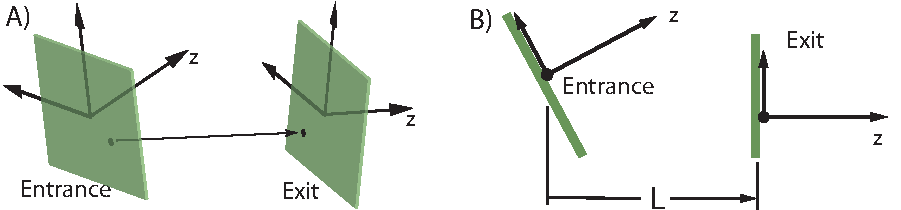
\includegraphics[width=5in]{patch.pdf}
  \caption[Standard patch transformation.]
{Standard tracking through a patch element. A particle's starting coordinate at
the entrance end of the patch has, by construction, coordinate $z$ =
0. The particle is drifted, as in a field free region, between the
entrance $z = 0$ plane and the exit $z = 0$ plane.}
  \label{f:patch.track}
\end{figure}

%---------------------------------------------------------------------------------

The transformation of the reference coordinates through a ``standard''
patch (a patch where custom fields are not used) is given by
\Eqs{vwlv} and \eq{wws}. At the entrance end of the patch, a
particle's position and momentum in the entrance coordinate system will be
\begin{alignat}{1}
  \bfr &= (x, y, 0) \CRNO
  \bfP &= (P_x, P_y, P_z) = 
    \left( p_x, p_y, \pm \sqrt{(1+p_z)^2 - p_x^2 - p_y^2} \right) \, P_{0\text{ent}}
\end{alignat}
where $p_x$, $p_y$ and $p_z$ are the phase space momenta, and $z$,
which is coordinate $z$ and not phase space $z$, is always zero by
construction as shown in \fig{f:patch.track} [Also see \fig{f:local.coords}
and the discussion in \sref{s:phase.space}.] The sign of the
longitudinal momentum $P_z$ is determined by whether the particle is
traveling in the positive $s$ or negative $s$ direction (which will
occur when an element is flipped longitudinally).

The transformation between entrance and exit coordinate systems is given by \Eqs{rwlr} and \eq{pps}
\begin{alignat}{1}
  \bfr &\rightarrow 
    \bfS^{-1} \, (\bfr - \bfL) \CRNO
  \bfP &\rightarrow \bfS^{-1} \, \bfP
\end{alignat}
where $\bf L$ is given by \Eq{lxyz}
\begin{example}
  \(\bf L\) =  (x_offset, y_offset, z_offset)
  \label{lxyz2}
\end{example}

After this transformation, the particle must be propagated by a longitudinal length
$-r_z$ to intersect the $r_z = 0$ plane of the exit face.
\begin{alignat}{1}
  \bfr &\rightarrow (r_x - r_z \, \frac{P_x}{P_z}, r_y - r_z \, \frac{P_y}{P_z}, 0) \CRNO
  \bfP &\rightarrow \bfP
\end{alignat}

The final $\bfr$ and $\bfP$ can now be used compute the particles
phase space coordinates, along with the time $t$ and the reference time
$t_{\text{ref}}$ at the exit end.
\begin{alignat}{3}
  x &\rightarrow r_x \qquad &p_x &\rightarrow \frac{P_x}{P_{0\text{exi}}} \CRNO
  y &\rightarrow r_y \qquad &p_y &\rightarrow \frac{P_y}{P_{0\text{exi}}} \\
  z &\rightarrow z + r_z \, \frac{|\bfP|}{P_z} + L_0 \, \frac{\beta}{\beta_0} +
    \beta \, \text{t_offset} \qquad
    &p_z &\rightarrow \frac{(1+p_z) \, P_{0\text{ent}} - P_{0\text{exi}}}{P_{0\text{exi}}} \CRNO
  t &\rightarrow t - r_z \, \frac{|\bfP|}{P_z \, \beta} \qquad
  &t_{\text{ref}} &\rightarrow t_{\text{ref}} + \text{t_offset} + L_0 \, \frac{1}{\beta_0} \nonumber
\end{alignat}
where the exit reference momentum $P_{0\text{exi}}$ is related to the
entrance reference momentum $P_{0\text{ent}}$ through
\vn{e_tot_offset}.  In the above equation, $\beta$ is the particle
velocity, $\beta_0$ is the velocity of the reference particle, and
$L_0$ is the drift length of the reference particle
\Begineq
  L_0 = \frac{1}{S^{-1}_{33}} \, \left( 
  S^{-1}_{31} \, \text{x_offset} + S^{-1}_{32} \, \text{y_offset} + S^{-1}_{33} \, \text{z_offset}
  \right)
\Endeq

%---------------------------------------------------------------------------------
%---------------------------------------------------------------------------------
\section{Quadrupole Element Tracking}
\label{s:quadrupole.std}
\index{quadrupole}

The \vn{bmad_standard} calculates the transfer map through an upright
quadrupole and then transforms that map to the laboratory frame.

The Hamiltonian for an upright quadrupole is
\Begineq
  H = \frac{p_x^2 + p_y^2}{2 (1 + p_z)} + \frac{k_1}{2} (x^2 - y^2)
\Endeq
This is simply solved
\begin{align}
  x_2    &= c_x \, x_1 + s_x \, \frac{p_{x1}}{1 + p_{z1}} \CRNO
  p_{x2} &= \tau_x \, \om^2 \, \, (1 + p_{z1}) \, s_x \, x_1 + c_x \, p_{x1} \CRNO
  y_2    &= c_y \, y_1 + s_y \, \frac{p_{y1}}{1 + p_{z1}} \CRNO
  p_{y2} &= \tau_y \, \om^2 \, \, (1 + p_{z1}) \, s_y \, y_1 + c_y \, p_{y1} \\
  z_2    &= z_1 + m_{511} \, x_1^2 + m_{512} \, x_1 \, p_{x1} + m_{522} \, p_{x1}^2 + 
                   m_{533} \, y_1^2 + m_{534} \, y_1 \, p_{y1} + m_{544} \, p_{y1}^2 \CRNO
  p_{z2} &= p_{z1} \nonumber
\end{align}
where 
\Begineq
  \om \equiv \sqrt{\frac{|k_1|}{1 + p_{z1}}}
\Endeq
and
\begin{alignat}{6}
         &\hspace*{3ex}  && k_1 > 0          &\hspace*{3ex}& k_1 < 0 & \qqquad
         &\hspace*{3ex}  && k_1 > 0          &\hspace*{3ex}& k_1 < 0 \CRNO
     c_x &=   && \cos  (\om \, L) && \cosh (\om \, L) & \qqquad
     c_y &=   && \cosh (\om \, L) && \cos  (\om \, L) \CRNO
     s_x &=   && \frac{\sin  (\om \, L)}{\om} && \frac{\sinh (\om \, L)}{\om} & \qqquad
     s_y &=   && \frac{\sinh (\om \, L)}{\om} && \frac{\sin  (\om \, L)}{\om} \\
  \tau_x &=   && {-}1             && {+}1             & \qqquad
  \tau_y &=   && {+}1             && {-}1             \nonumber
\end{alignat}
with this
\begin{alignat}{2}
  m_{511} &= \frac{\tau_x \,\, \om^2}{4} \, (L - c_x \, s_x) & \qqquad
  m_{533} &= \frac{\tau_y \,\, \om^2}{4} \, (L - c_y \, s_y) \CRNO
  m_{512} &= \frac{-\tau_x \,\, \om^2}{2 \, (1 + p_{z1})} \, s_x^2 & \qqquad
  m_{534} &= \frac{-\tau_y \,\, \om^2}{2 \, (1 + p_{z1})} \, s_y^2 \\
  m_{522} &= \frac{-1}{4 \, (1 + p_{z1})^2} \, (L + c_x \, s_x) & \qqquad
  m_{544} &= \frac{-1}{4 \, (1 + p_{z1})^2} \, (L + c_y \, s_y) \nonumber
\end{alignat}

%---------------------------------------------------------------------------------
%---------------------------------------------------------------------------------
\section{RFcavity Element Tracking}
\label{s:rfcavity.std}
\index{rfcavity}

Tracking through an rfcavity uses a kick-drift-kick model. The kick is
a pure energy kick (see equations in \sref{s:rfcav}) and the phase of
the RF is calculated under the assumption that the waveform moves at a
phase velocity equal to the velocity of the reference particle.

\index{lcavity}
The transverse forces due to the RF are ignored. This is a resonable
approximation when the acceleration is small. \vn{Lcavity} elements
should be used in place of \vn{rfcavity} elements when this is not so.

%---------------------------------------------------------------------------------
%---------------------------------------------------------------------------------
\section{Sextupole Element Tracking}
\label{s:sextupole.std}
\index{sextupole}

The Hamiltonian for an upright sextupole is
\Begineq
  H = \frac{p_x^2 + p_y^2}{2 (1 + p_z)} + \frac{k_2}{6} (x^3 - 3 \, x \, y^2)
\Endeq

Tracking through a sextupole uses a kick-drift-kick model.

%---------------------------------------------------------------------------------
%---------------------------------------------------------------------------------
\section{Sol\_Quad Element Tracking}
\label{s:sol.quad.std}
\index{sol_quad}

The Hamiltonian is
\Begineq
  H = \frac{(p_x + \frac{k_s }{2}\, y)^2}{2 (1 + p_z)} + 
  \frac{(p_y - \frac{k_s}{2} \, x)^2}{2 (1 + p_z)} + \frac{k_1}{2} (x^2 - y^2)
\Endeq
Solving the equations of motion gives
\begin{align}
  x_2    &= m_{11} \, x_1 + m_{12} \, p_{x1} + m_{13} \, y_1 + m_{14} \, p_{y1} \CRNO
  p_{x2} &= m_{21} \, x_1 + m_{22} \, p_{x1} + m_{23} \, y_1 + m_{24} \, p_{y1} \CRNO
  y_2    &= m_{31} \, x_1 + m_{32} \, p_{x1} + m_{33} \, y_1 + m_{34} \, p_{y1} \CRNO
  p_{y2} &= m_{41} \, x_1 + m_{42} \, p_{x1} + m_{43} \, y_1 + m_{44} \, p_{y1} \\
  z_2    &= z_1 + \sum_{j = 1}^4 \sum_{k = j}^4 m_{5jk} \, r_j \, r_k  \CRNO
  p_{z2} &= p_{z1} \nonumber
\end{align}
where
\begin{alignat}{2}
  m_{11} &= \frac{1}{2 \, f} \, \left( f_{0+} \, c + f_{0-} \, c_h \right) & \qqquad
  m_{31} &= -m_{24} \CRNO
  m_{12} &= \frac{1}{2 \, f \, (1 + p_{z1})} \, 
            \left( \frac{f_{++}}{\om_+} \,  s + \frac{f_{--}}{\om_-} \, s_h \right) & \qqquad
  m_{32} &= -m_{14} \CRNO
  m_{13} &= \frac{\ks}{4 \, f} \, 
            \left( \frac{f_{+-}}{\om_+} \, s +\frac{f_{-+}}{\om_-} \, s_h \right) & \qqquad
  m_{33} &= \frac{1}{2 \, f} \, \left( f_{0-} \, c + f_{0+} \, c_h \right) \CRNO
  m_{14} &= \frac{\ks}{f \, (1 + p_{z1})} \, \left( -c + c_h \right) & \qqquad
  m_{34} &= \frac{1}{2 \, f \, (1 + p_{z1})} \, 
            \left( \frac{f_{+-}}{\om_+} \, s + \frac{f_{-+}}{\om_-} \, s_h \right) \CRNO
  m_{21} &= \frac{-(1 + p_{z1})}{8 \, f} \, 
            \left( \frac{\xi_{1+}}{\om_+} \, s + \frac{\xi_{2+}}{\om_-} s_h \right) & \qqquad
  m_{41} &= -m_{23} \\
  m_{22} &= m_{11} & \qqquad
  m_{42} &= -m_{13} \CRNO
  m_{23} &= \frac{\ks^3 \, (1 + p_{z1})}{4 \, f} \, \left( c - c_h \right) & \qqquad
  m_{43} &= \frac{-(1 + p_{z1})}{8 \, f} \, 
            \left( \frac{\xi_{1-}}{\om_+} \, s + \frac{\xi_{2-}}{\om_-} \, s_h \right) \CRNO
  m_{24} &= \frac{\ks}{4 \, f} \, 
            \left( \frac{f_{++}}{\om_+} \, s + \frac{f_{--}}{\om_-} \, s_h \right) & \qqquad
  m_{44} &= m_{33} \nonumber
\end{alignat}
and
\begin{alignat}{2}
  \kone        &= \frac{k_1}{1 + p_{z1}} & \qqquad 
  \ks          &= \frac{k_s}{1 + p_{z1}} \CRNO
  f            &= \sqrt{\ks^4 + 4 \, \kone^2} & \qqquad
  f_{\pm0}     &= f \pm \ks^2 \CRNO
  f_{0\pm}     &= f \pm 2 \, \kone & \qqquad
  f_{\pm\pm}   &= f \pm \ks^2 \pm 2 \, \kone \CRNO
  \om_+        &= \sqrt{\frac{f_{+0}}{2}} & \qqquad
  \om_-        &= \sqrt{\frac{f_{-0}}{2}} \\
  s            &= \sin (\om_+ \, L) & \qqquad
  s_h          &= \sinh (\om_- \, L) \CRNO
  c            &= \cos (\om_+ \, L) & \qqquad
  c_h          &= \cosh (\om_- \, L) \CRNO
  \xi_{1\pm} &= \ks^2 \, f_{+\mp} \pm 4 \, \kone \, f_{+\pm} & \qqquad
  \xi_{2\pm} &= \ks^2 \, f_{-\pm} \pm 4 \, \kone \, f_{-\mp} \nonumber
\end{alignat}

The $m_{5jk}$ terms are obtained via \Eq{zz121p}
\begin{align}
  m_{5jk} = - \frac{\tau_{jk}}{2 (1 + p_{z1})^2} \int \! ds \, 
  & \left[ 
    \left( m_{2j} + \frac{k_s}{2} \, m_{3j} \right) \, 
    \left( m_{2k} + \frac{k_s}{2} \, m_{3k} \right)   
  \right. + \\
  & \hspace*{15ex} \left.
    \left( m_{4j} - \frac{k_s}{2} \, m_{1j} \right) \, 
    \left( m_{4k} - \frac{k_s}{2} \, m_{1k} \right) 
  \right] \nonumber
\end{align}
where
\Begineq
  \tau_{jk} = 
  \begin{cases}
    1 & j = k \\
    2 & j \ne k 
  \end{cases}
\Endeq
The needed integrals involve the product of two trigonometric or
hyperbolic functions. These integrals are trivial to do but the
explicit equations for $m_{5jk}$ are quite long and in the interests of
brevity are not reproduced here.

%---------------------------------------------------------------------------------
%---------------------------------------------------------------------------------
\section{Solenoid Element Tracking}
\label{s:solenoid.std}
\index{solenoid}

The Hamiltonian is
\Begineq
  H = \frac{ \left( p_x + \frac{k_s}{2} \, y \right)^2}{2 \, (1 + p_z)} + 
  \frac{ \left( p_y - \frac{k_s}{2} \, x \right)^2}{2 \, (1 + p_z)} 
\Endeq
The solution is
\begin{align}
  x_2    &= \frac{1 + c}{2} \, x_1 + \frac{s}{k_s} \, p_{x1} +
           \frac{s}{2} \, y_1 + \frac{1 - c}{k_s} \, p_{y1} \CRNO
  p_{x2} &= \frac{-k_s \, s}{4} \, x_1 + \frac{1 + c}{2} \, p_{x1} - 
           \frac{k_s \, (1 - c)}{4} \, y_1 + \frac{s}{2} \, p_{y1} \CRNO
  y_2    &= \frac{-s}{2} \, x_1 - \frac{1 - c}{k_s} \, p_{x1} +
           \frac{1 + c}{2} \, y_1 + \frac{s}{k_s} \, p_{y1} \\      
  p_{y2} &= \frac{k_s \, (1 - c)}{4} \, x_1 + \frac{-s}{2} \, p_{x1} -
            \frac{k_s \, s}{4} \, y_1 + \frac{1 + c}{2} \, p_{y1} \CRNO 
  z_2    &= z_1 + \frac{L}{2 \, (1 + p_{z1})^2} \, 
                   \left[ \left( p_{x1} + \frac{k_s}{2} \, y_1 \right)^2 +
                          \left( p_{y1} - \frac{k_s}{2} \, x_1 \right)^2 \right] \CRNO
  p_{z2} &= p_{z1} \nonumber
\end{align}
where
\begin{align}
  c &= \cos \left( \frac{k_s}{2} \, L \right) \CRNO
  s &= \sin \left( \frac{k_s}{2} \, L \right)
\end{align}

Effectively, with this formulation, the fringe fields form
